\documentclass[paper=a4, fontsize=9pt]{article}
\usepackage[utf8]{inputenc}

\usepackage[a4paper]{geometry}
\geometry{top=2cm, bottom=2cm, left=2cm, right=2cm}
\setlength{\parskip}{2mm}

\usepackage{lipsum}

\usepackage[spanish]{babel}										
\usepackage[protrusion=true,expansion=true]{microtype}		    % Better typography
\usepackage{amsmath,amsfonts,amsthm}					                % Math packages
\usepackage[pdftex]{graphicx}									                % Enable pdflatex
\usepackage[svgnames]{xcolor}									                % Enabling colors by their 'svgnames'
\usepackage[hang, small, labelfont=bf,up,textfont=it,up]{caption}	% Custom captions under/above floats
\usepackage{epstopdf}											  	                % Converts .eps to .pdf
\usepackage{subfig}												  	                % Subfigures
\usepackage{wrapfig}
\usepackage{float}
\usepackage{booktabs}											  	                % Nicer tables
\usepackage{fix-cm}												  	                % Custom fontsizes
\usepackage{hyperref}                                         % Link Clicks
\usepackage{filecontents}



%opening
\title{Métodos estadísticos aplicados al baloncesto}
\author{Paula Moreno Blazquez}
\date{Enero 2022}

\usepackage{Sweave}
\begin{document}
\Sconcordance{concordance:TFG_MetodosEstadisticosBaloncesto.tex:TFG_MetodosEstadisticosBaloncesto.Rnw:%
1 31 1 1 0 226 1 1 34 16 0 1 51 37 0 1 208 2 0 1 31 1 2 44 1 1 2 1 0 18 %
1 1 3 1 0 1 5 3 0 1 3 1 0 1 3 19 0 1 3 1 0 1 5 3 0 2 2 1 0 2 2 1 0 2 2 %
1 0 2 2 1 0 2 2 1 0 2 2 1 0 2 2 1 0 2 2 1 0 2 2 1 0 2 2 1 1 1 2 41 0 1 %
2 2 1 1 3 2 0 2 1 1 7 5 0 1 2 1 7 5 0 1 2 1 1 1 3 4 0 1 2 10 1 1 7 6 0 %
1 5 6 0 1 2 4 1}


\maketitle

\clearpage

\begin{abstract}

Hoy en día, el deporte es un hobby muy popular por todo el mundo. Desde pequeños, los niños practican algún tipo de deporte, especialmente aquellos que son de equipo. Eso nos lleva a querer saber más del deporte, más detalles, más información. Nos entra la curiosidad de "¿quién es el mejor jugador?", "Qué equipo es mejor?", o incluso intentar prevenir qué equipo ganará según sus resultados anteriores. Y gracias a los avances tecnológicos e informáticos, cada vez se nos facilita más poder seguir un deporte desde casa, ver la estadística de los deportistas e incluso hay plataformas o juegos que nos permiten ser, de manera virtual, managers de los clubs y, por lo tanto, nos facilitan mucha información que antes era más difícil de saber.

Eso hace que, de manera progresiva, también mejore el estudio y el análisis de cada deporte, y cada vez sea más específica para cada deporte, implementando nuevos recursos para mejorar los resultados. Pero, ¿son lo suficientemente eficaces los análisis que se realizan actualmente en Europa? ¿O dichos análisis están anticuados y requieren de una actualización?

\end{abstract}

\pagebreak            
\newpage              

\tableofcontents

\clearpage



\section{Introducción}

En este trabajo estudiaremos más a fondo el Baloncesto, el segundo deporte más popular de Europa (solo superado por el futbol), y el cual tengo interés personal, ya que lo practico desde los 4 años.

Esta idea de estudio surgió del constante pensamiento de que los análisis actuales que se hacen en este deporte en Europa son bastante pobres a nivel informativo, puesto que se basan en conceptos muy básicos, y principalmente ofensivos (que vendría a ser el 50\% de un partido). Para que nos hagamos una idea, el estadístico por preferencia es el llamado \emph{Valoración} y que se originó en 1991 (hace 30 años) y desde entonces nunca se ha modificado.

Es por eso que, considero que actualmente los análisis que se hacen de este deporte necesitan una actualización significativa para llegar a informar de todos aquellos datos que hoy en día si se pueden recoger gracias a los avances tecnológicos, y de los cuales no se analizan por falta de dinero o porque se consideran poco relevantes.

El objetivo principal de este estudio es mejorar los análisis que se elaboran de cada partido, para poder encontrar una variable respuesta que nos diga que aportación al equipo tiene cada jugador personalmente, disminuyendo la diferencia de pesos que hay actualmente entre las aportaciones ofensivas y las aportaciones defensivas.

Este documento se estructura de la siguiente manera: a continuación, se realizará una breve explicación de los recursos informáticos que se han utilizado para realizar este estudio, seguidamente se explicará brevemente los conceptos de baloncesto que son necesarios para entender los tecnicismos del trabajo y se presentaran posibles análisis que se realizan. Finalmente, se describirá la base de datos con la que se ha trabajado y sus variables, y también se explicará en profundidad el análisis que se desarrollará en este trabajo, el Más/Menos Ajustado (\emph{Adjusted Plus/Minus, APM}). En la sección de resultados presentaremos la resolución del análisis y finalmente discutiremos, en la sección de conclusiones, los resultados obtenidos.
\section{El baloncesto}

\subsection{Historia y reglas básicas}

\begin{wrapfigure}{r}{0.3\linewidth}
\centering
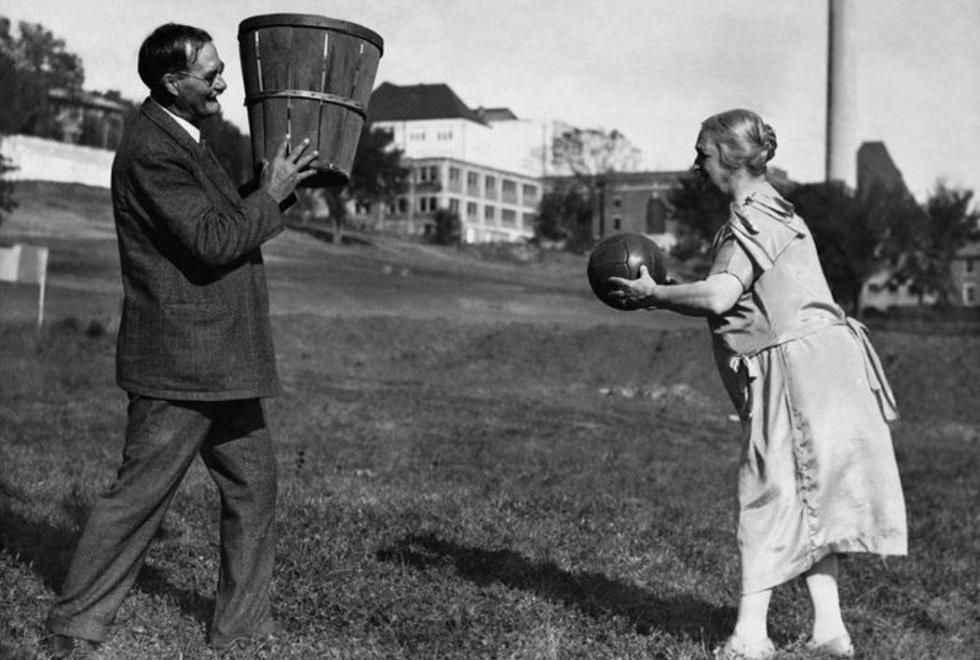
\includegraphics[width=0.3\textwidth]{imagenes/historia_baloncesto.jpg}
\label{fig:hist_bskb}
\end{wrapfigure}

El baloncesto es un deporte de equipo que se originó en 1891, por James Naismith, profesor de educación física en la escuela YMCA de Springfield, Massachusetts, Estados Unidos.

James buscaba idear un deporte que sus alumnos pudieran practicar bajo techo, pues los duros inviernos en Massachusetts dificultaban la realización de ejercicio al aire libre, por lo que inventó el baloncesto utilizando unas cajas de melocotones y unos balones.

Con el paso de los años, este deporte, que empezó como actividad de colegio, ha ido evolucionando mucho, añadiendo más reglas, conceptos nuevos, límites de números de jugadores, se ha determinado tiempos de juego, las canastas tienen un valor distinto según la distancia, etc.

Actualmente, las normas más básicas de este deporte son:

\begin{itemize}

\item En las ligas superiores, hay un total de 4 cuartos de 10 minutos y pueden estar en pista 5 jugadores por equipo.
\item No te puedes desplazar con la pelota en las manos, es obligatorio botar con una mano (si no será una infracción y conllevará la perdida de pelota y saque de banda del equipo rival).
\item Cada jugador puede realizar hasta un total de 5 faltas, que será penalizado con un saque de banda o con un tiro libre (dependerá de la situación). El jugador que ejecuta 5 faltas será expulsado del partido.
\item El objetivo es encestar el máximo de puntos posibles, teniendo en cuenta que pueden sumar 1, 2 o 3 puntos, según la distancia.

\end{itemize}

\clearpage

\subsection{Conceptos y definiciones básicas del baloncesto:}

Para que podamos entender a que nos referimos en este trabajo, es necesario comprender unos conceptos básicos de vocabulario. Tendremos en cuenta los conceptos que se necesitan para realizar la valoración del jugador y/o del equipo que se utilizan en las estadísticas federadas.

\begin{itemize}

\item Puntos: Acumulación de tiros encestados multiplicados por su valor, que cada jugador y/o equipo realiza durante el partido
\item Minutos: Número de minutos que el jugador está en pista
\item Falta: Acción en la que un defensor bloquea el avance de su rival sin tener control de balón o de manera no reglamentaria (empujar, agarrar...)
\item Pérdidas de balón: cuando un equipo pierde el control del balón y pasa a ser del equipo rival.
\item Rebotes: Recuperación de pelota después de que el tiro sea ejecutado, pero no haya encestado.
\item Recuperación de balón: Cuando un equipo consigue robar el balón al equipo rival.
\item Asistencia: Es un pase a un jugador que se encuentra en una posición de ventaja o que le ayuda a conseguir una canasta sin hacer ningún bote.
\item Tapón: Bloqueo de un tiro en el aire.

\end{itemize}

\section{Posibles análisis realizables en el baloncesto}

Viendo la gran cantidad de datos que se pueden extraer de cada partido (y de cada equipo), se han ido creando análisis que recogen estos datos y los analizan para ayudarnos a identificar y desarrollar hipótesis sobre cada jugador y/o equipo.

\subsection{Boxscore}

El primer análisis que se hizo fue un \emph{Box Score} (Caja de puntuación) donde se recopilaba únicamente los puntos de cada jugador según el valor de esta y las faltas realizadas. Posteriormente, se fue mejorando añadiendo conceptos como rebotes, tapones, pérdidas de balón, recuperaciones de balón... Y se añadió el estadístico (que actualmente es por defecto) que se hace a partir de todos estos datos: \emph{Valoración} (en inglés PIR, \emph{Performance Index Rating}) que engloba todo lo básico que pasa en el partido de manera individual y que, cuanto más positivo, mejor. Este estadístico se calcula utilizando la siguiente fórmula:

\begin{equation} \label{eq1}
\begin{split}
PIR = & (Puntos + Rebotes + Asistencias + Robos + Tapones + Faltas Recibidas) - \\
& (Tiros de Campo Fallados + Tiros Libres Fallados + Tapones Recibidos + Pérdidas + Faltas Realizadas)
\end{split}
\end{equation}

\centerline{(en el \hyperref[sec:Anexo1]{Anexo 1} encontraréis la descripción de cada variable)}

\vspace{0.2cm}

Posteriormente, se añadió la variable "Más/Menos" (\emph{P/M, Plus/Minus}) que tiene que ver con la diferencia de puntos en el marcador durante el tiempo que el jugador esté en pista. Esta variable sirve para ver la contribución de los jugadores cuando están en pista. Todos los jugadores parten inicialmente con un 0, y según van entrando y saliendo de la pista, esta variable se va actualizando. Por ejemplo, los jugadores que son del quinteto inicial, empiezan con el marcador 0 - 0, y un $P/M = 0$. Si en el minuto 5, se substituye un jugador en cancha del equipo local (J1) por otro que está descansando (J2), y el marcador va 12 - 7, el $P/M$ del J1 pasará a ser $+5$. Y si al cabo de 3 minutos, se sustituye el J2 por otro (J3) y el marcador ahora va 20 - 9, el $P/M$ del J2 será $+6$ ($(20-12) - (9-7) = 8 - 2 = +6$).

\begin{figure}[H]
\centering
\begin{minipage}{.5\textwidth}
\centering
\captionsetup{width=.8\linewidth}
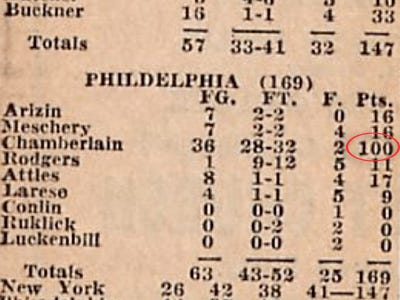
\includegraphics[width=.8\linewidth]{imagenes/BoxScore1962.jpg}
\captionof{figure}{Boxscore del partido de la NBA de Philadelphia Warriors contra New York Knicks, del 2 de Marzo de 1962}
\label{fig:BoxScore1962}
\end{minipage}%
\begin{minipage}{.5\textwidth}
\centering
\captionsetup{width=.8\linewidth}
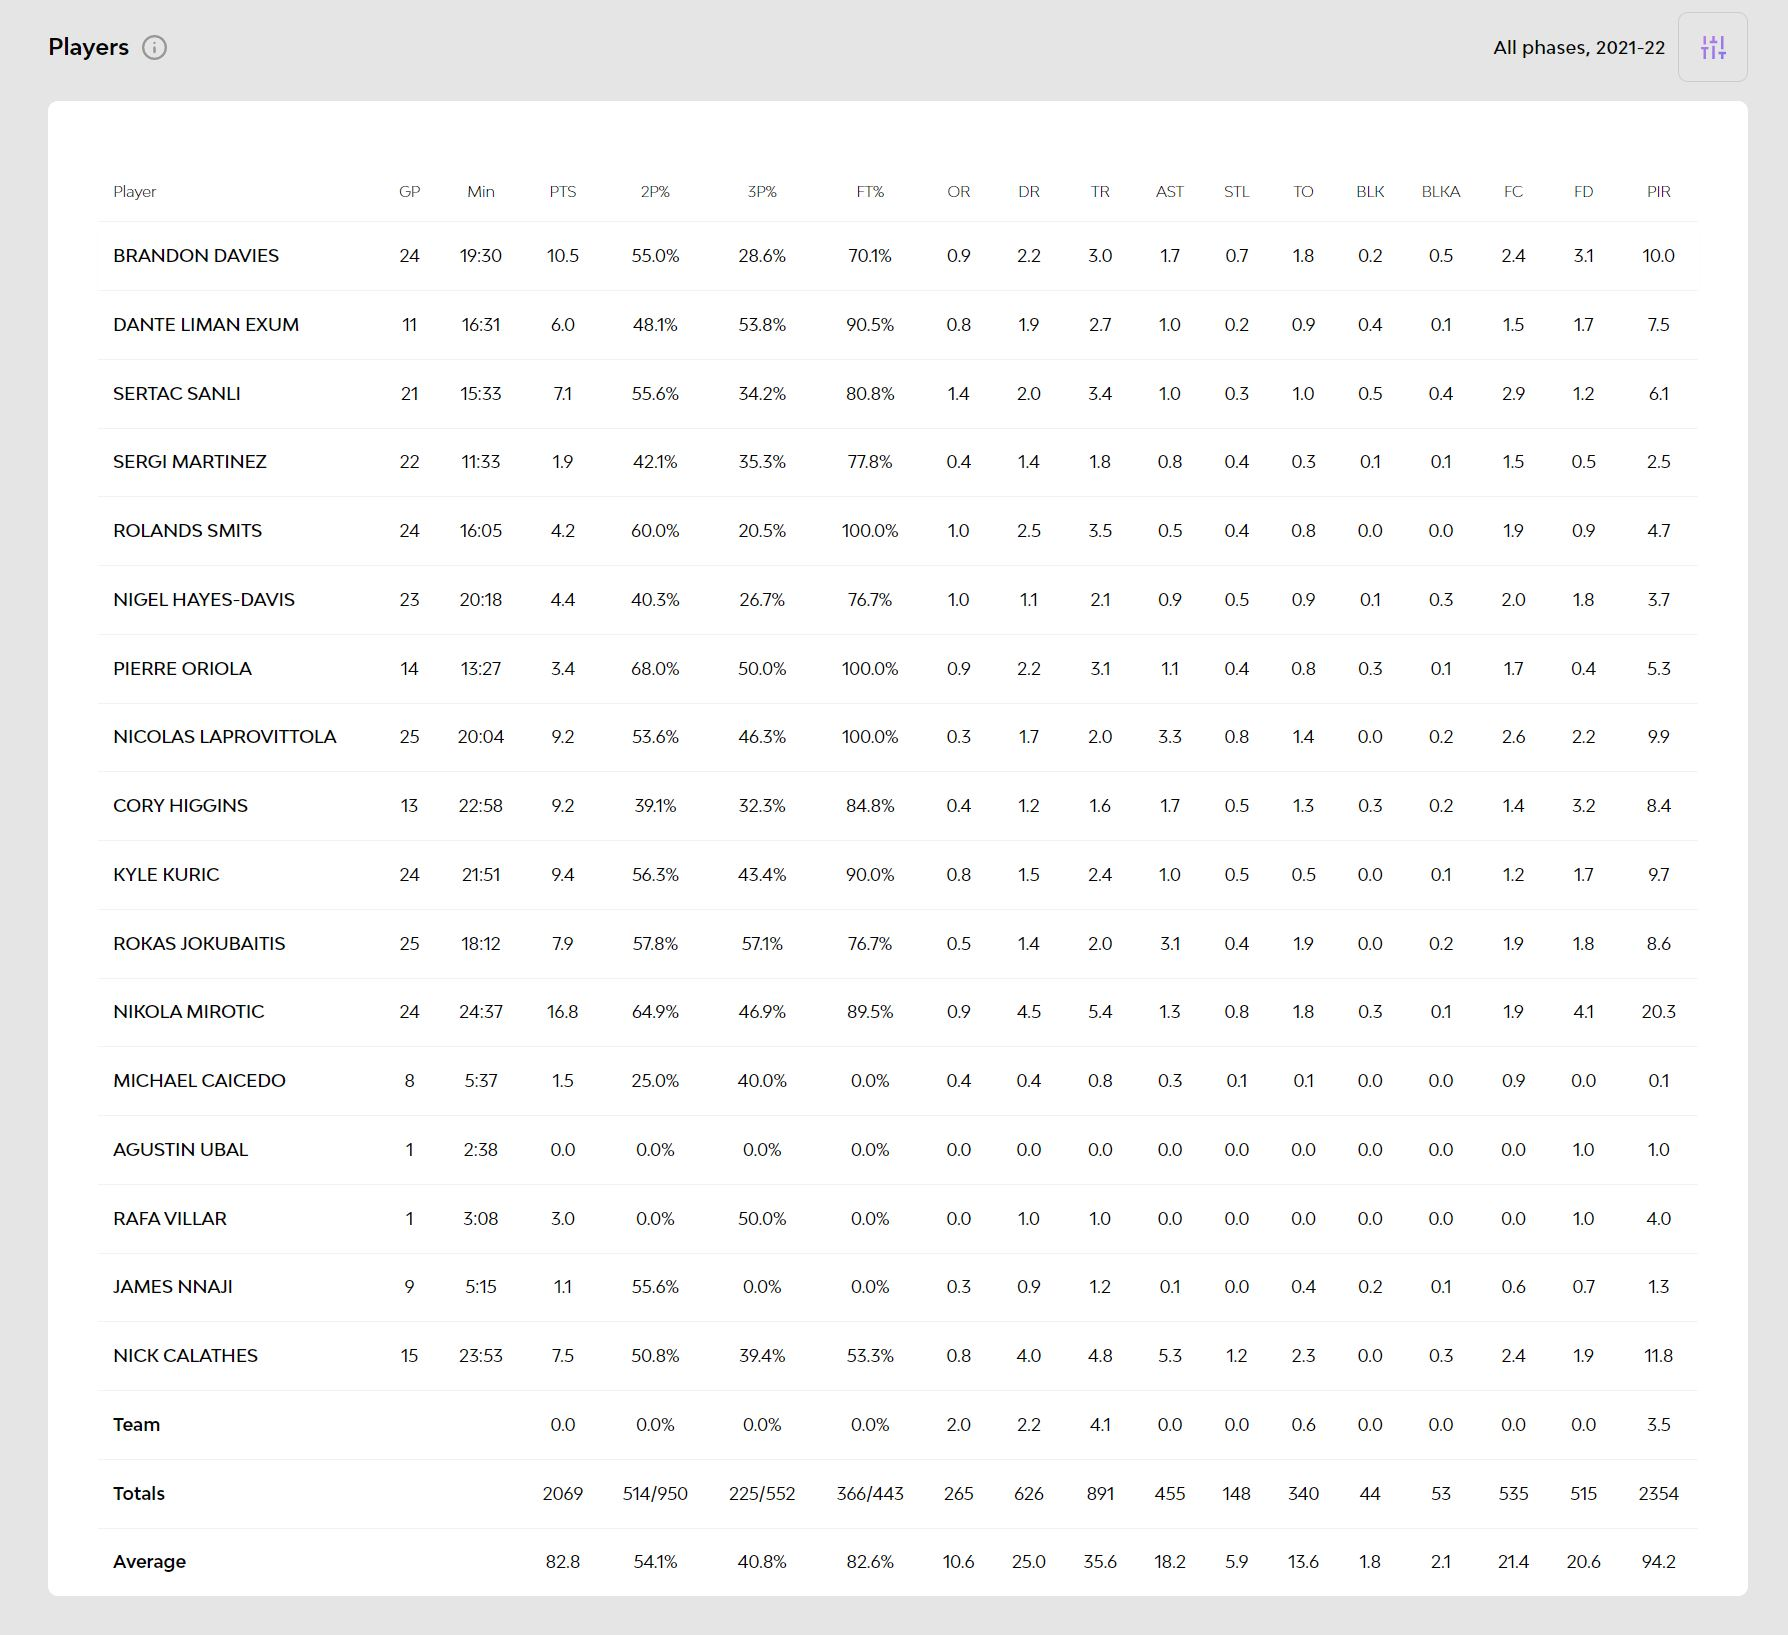
\includegraphics[width=.7\linewidth]{imagenes/BoxScore2022.jpg}
\captionof{figure}{Boxscore del partido de la Euroliga de Real Madrid contra FC Barcelona, del 11 de Febrero del 2022}
\label{fig:BoxScore2022}
\end{minipage}
\end{figure}

Aunque un \emph{Box Score} es muy útil para realizar análisis básicos, ya que es muy visual y cualquier persona sin la necesidad de muchos recursos puede analizar y predecir ciertos valores, pero estadísticamente perdemos una parte importante de la información de los datos, puesto que no nos los muestra progresivamente, sino que nos da los valores acumulados al final del tiempo establecido, y muchas veces contiene información engañosa, especialmente en las estadísticas defensivas.

Por lo que, para el desarrollo temporal del partido y para conocer cierta información de equipo que piden entrenadores y clubs, no nos sirve (como por ejemplo la eficacia de los quintetos, el desarrollo del marcador o de cualquier otra variable del equipo entero durante un tiempo determinado del partido, etc.)



\subsection{Play-by-play}

\begin{wrapfigure}{r}{0.4\linewidth}
\centering
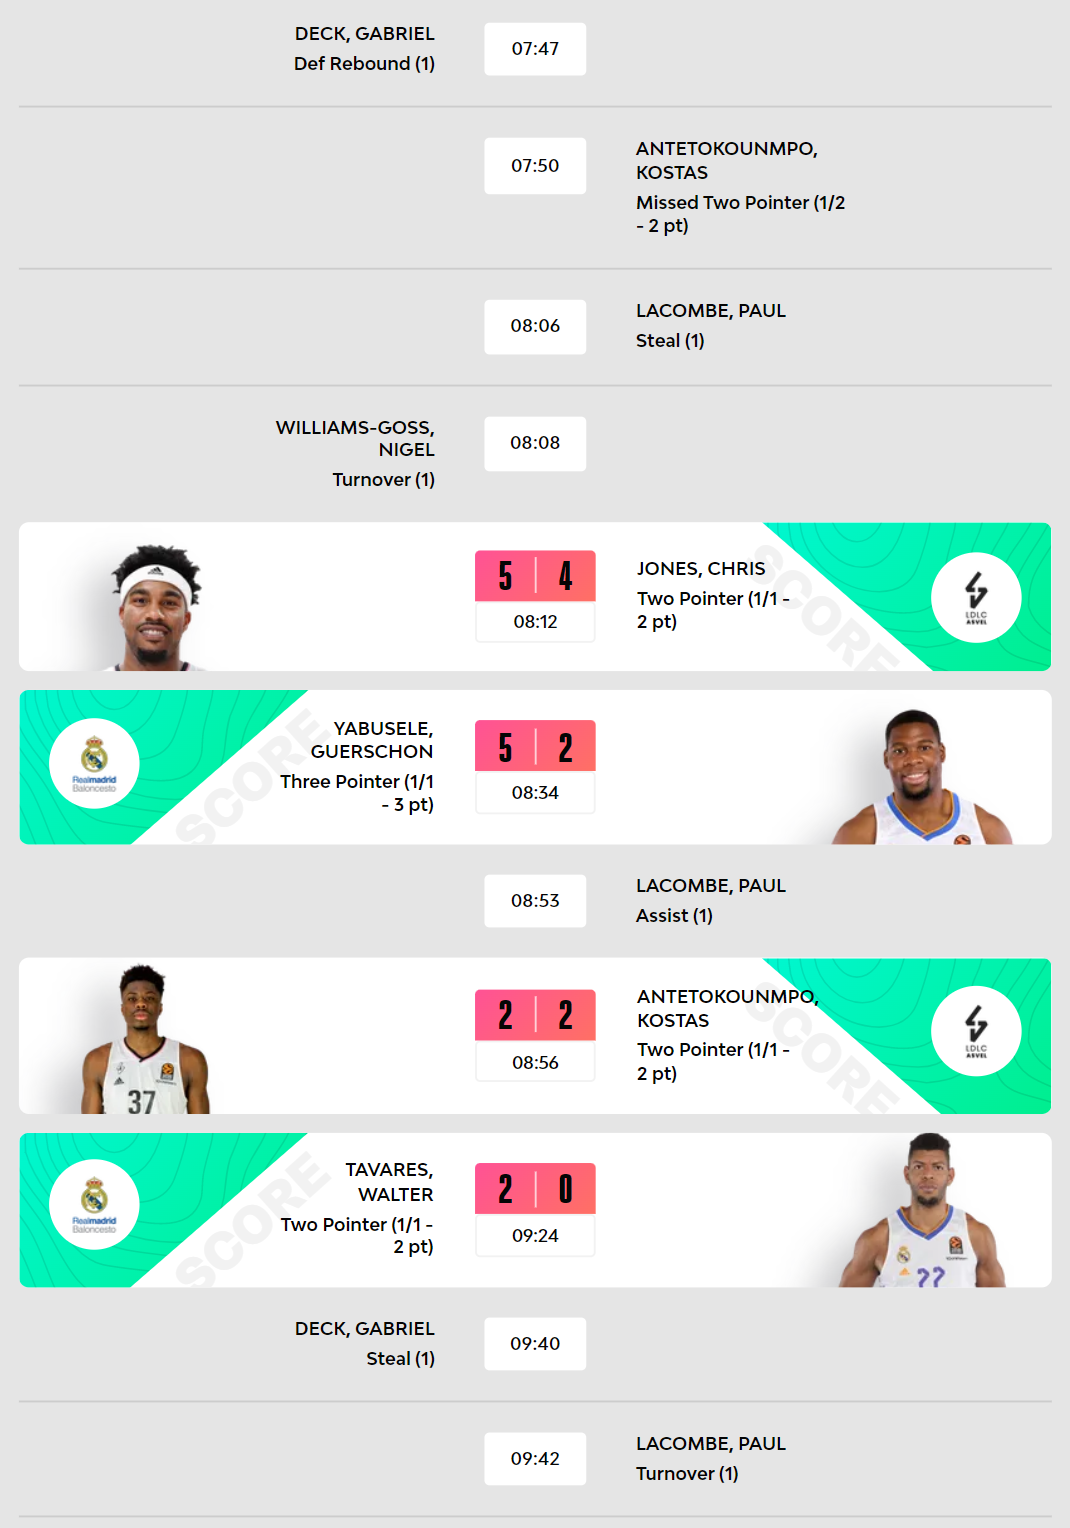
\includegraphics[width=0.4\textwidth]{imagenes/PBP_RM.png}
\captionsetup{width=.9\linewidth}
\captionof{figure}{\emph{Play by play} del partido de la Euroliga de Real Madrid contra LDLC Asvel, del 17 de Marzo del 2022. Se lee de abajo hacia arriba.}
\label{fig:PBP_RM}
\end{wrapfigure}

Este tipo de recogida de información se creó para solucionar el problema que teníamos con el \emph{Box Score}. Los datos de \emph{Play-by-Play (PBP)} han sido la fuente principal de muchas estadísticas avanzadas, como el más-menos ajustado, que se desarrollará en este trabajo.

\emph{Play-by-Play} proporciona una transcripción del juego en un formato de eventos individuales. Los datos típicos de jugada por jugada deben tener la siguiente información:

\begin{itemize}
\item El tiempo de la posesión
\item El jugador que inició la posesión (en caso de robo o rebote defensivo)
\item El jugador contrario que inició la posesión (en caso de un tiro fallado o pérdida de balón), incluida la ubicación en el piso desde donde se realizó el tiro y algunos otros identificadores únicos que usamos para clasificar el tipo de posesión.
\end{itemize}

Este tipo de análisis se inicializaron en 2007 para la Euroliga (principal competición europea de baloncesto) y en 2012 para la Eurocopa (competición internacional de segundo nivel).

\clearpage

\subsection{Shot-charts}

Este tipo de análisis es de los más visuales, ya que se realiza de una manera muy sencilla: se tiene como plantilla el dibujo de una pista de baloncesto de manera vectorial, y se va colocando cada tiro realizado en la posición del tiro, el jugador y si se encesta o no. De forma general se hace escribiendo el número del jugador en la posición desde donde se ejecuta el tiro, y si encesta, se hace un círculo alrededor del número.

El \emph{Shot-Charts}, proporciona un output visual muy fácil de interpretar, ya que es se parece a un mapa de calor y, por lo tanto, podemos observar de una manera muy rápida desde que zonas de la pista es más efectivo el equipo y/o el jugador.

Una vez realizado, podemos obtener con facilidad el porcentaje de acierto del equipo y/o el jugador, o incluso, determinar el porcentaje de acierto por zonas.

De este análisis, es frecuente encontrar variantes: mapa de calor del equipo, mapa de porcentajes de aciertos por zonas de la pista...

\begin{figure}[H]
\centering
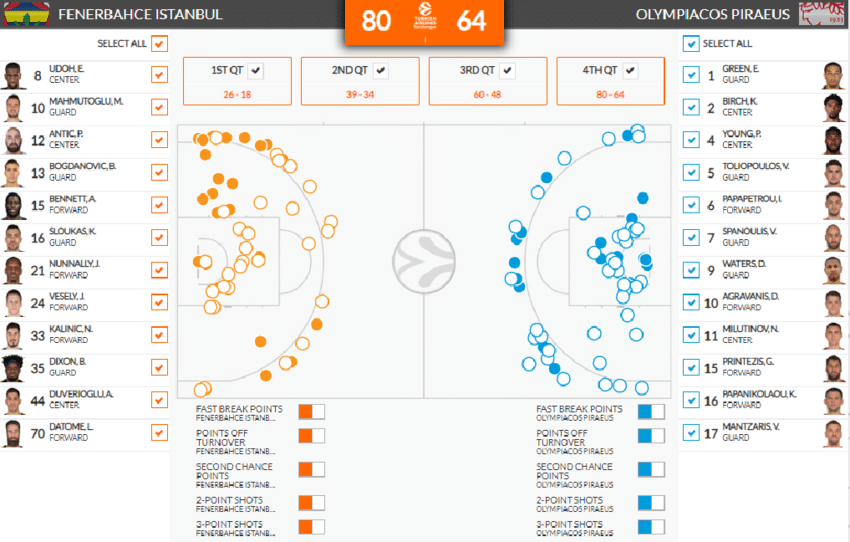
\includegraphics[width=.5\linewidth]{imagenes/shot_chart_1.png}
\captionof{figure}{\emph{Shot-Chart} del partido de la Euroliga del Fenerbahce Istanbul contra Olympiacos Piraeus, del 21 de Mayo del 2021.}
\label{fig:SC_FO}
\end{figure}


\subsection{Graphic Stats}

Este tipo de análisis es más moderno y se centra en un único equipo o (más frecuentemente) en un jugador, y se visualiza sus números de manera muy visual y con mucho carácter para marketing y fáciles de compartir en redes sociales.

Básicamente, consiste en, de manera creativa y con un diseño moderno, enseñar los números que ha realizado dicho jugador. Normalmente, se visualiza puntos, rebotes y asistencias o si no también se suele mostrar el porcentaje de acierto en los diferentes tiros, conjuntamente con una o varias fotografías del jugador.

La información de este tipo de análisis viene obtenida de alguna de los anteriores tipos, por lo tanto, aunque se considera un análisis deportivo, es más bien una representación gráfica y visual de los datos destacados del jugador o del equipo.

\begin{figure}[H]
\centering
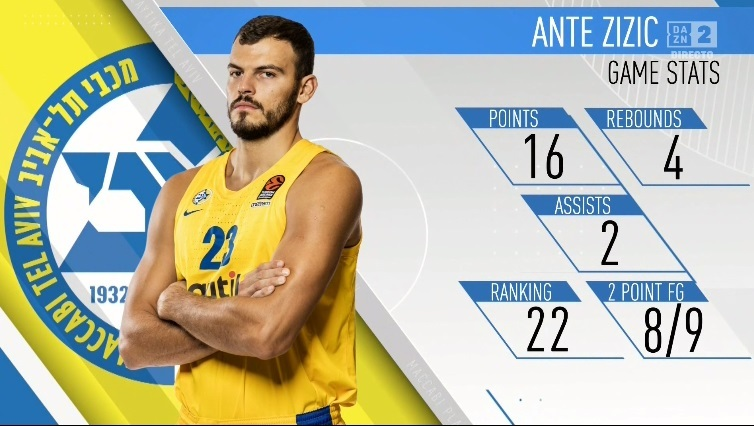
\includegraphics[width=.5\linewidth]{imagenes/GraphicStat.jpg}
\captionof{figure}{\emph{Graphic Stats} de Ante Zizic, jugador de Maccabi Tel Aviv en el partido del contra el FC Barcelona del 30 de Marzo de 2021.}
\label{fig:GS_AZ}
\end{figure}


\clearpage

\section{Estadístico Más/Menos (\emph{Plus/Minus})}

Como ya hemos comentado, el Más/Menos ($+/-$, $\pm$) es una estadística deportiva utilizada para medir el impacto de un jugador en el juego. Conforme se ha ido conociendo y estudiando más este estaístico, se ha revelado que tiene fallas o que no es tan preciso, por lo que confiar únicamente en el Más/Menos es un gran error, por eso se han desarrollado y han tratado de reducir estas fallas para intentar obtener resultados más precisos con respecto al impacto de un jugador. Actualmente, se están publicando diferentes tipos de métricas sobre el Más/Menos:

\subsection{Plus Minus, PM}

Este es el estadístico original que está representado por la diferencia entre la puntuación total de su equipo y la de su oponente cuando el jugador está en el juego. Se basa únicamente en la información del marcador de baloncesto tradicional; no se incluyen datos \emph{play-by-play} ni datos de cuadro de puntuación no tradicionales (como mates o robos).

Fueron Los Montreal Canadiens de la NHL (hockey sobre hielo) el primer equipo en medir el más-menos de sus jugadores, comenzando en algún momento de la década de 1950. Aunque es estadístico fue pionero en el hockey, se ha utilizado en otros deportes y áreas de la vida, llegando al mundo del baloncesto por los Houston Rockets de la NBA, que lo utilizaron por primera vez una versión modificada de la estadística, que ayudó a revelar la efectividad no anunciada de Shane Battier, quien anotó muy poco. Ahora es de uso regular en toda la NBA. 

Se calcula de la diguiente manera:

$$PM_i = PointsTeam - PointsOpponent$$

\subsection{Adjusted Plus Minus, APM}

Plus-Minus ajustado (a menudo abreviado APM) es un análisis de baloncesto que intenta predecir el impacto de un jugador individual en el margen de puntuación de un juego mediante el control del resto de los jugadores en la cancha en un momento dado. La métrica se deriva utilizando datos jugada por jugada para realizar un seguimiento de todas las acciones de finalización de sustitución y posesión. Los Dallas Mavericks lo implementaron por primera vez a principios de la década de 2000 después de que el propietario Mark Cuban encargara a los científicos de datos Jeff Sagarin, Wayne Winston y Dan Rosenbaum, quienes desarrollaron la métrica junto con su conversión WINVAL para ayudar en la determinación del salario de los jugadores.[1] En combinación con otras innovaciones, esto le dio a los Mavericks una de las oficinas centrales más progresistas de la liga en ese momento. Desde la creación de APM, se han creado varias métricas derivadas que intentan mejorar el esqueleto.

\subsection{Regularized Adjusted Plus/Minus, RAPM}

\subsection{Real Plus-Minus, RPM}

\subsection{Otros tipos de métricas basados en el Más/Menos}

\begin{itemize}
\item Defensive Plus-Minus aka DPM
\item Net Plus-Minus aka Roland Rating
\item Adjusted Plus-Minus aka APM por Wayne Winston and Jeff Sagarin
\item Statistical Plus-Minus aka SPM por Dan Rosenbaum
\item Regularized Adjusted Plus-Minus aka RAPM por Joe Sill
\item Real Plus-Minus aka RPM por ESPN (basado en el tranajo de Steve Ilardi y Jeremias Engellmann)
\item Box Plus-Minus aka BPM por Daniel Myers
\item Player Tracking Plus-Minus aka PT-PM
\item Estimated Plus-Minus aka EPM por Taylor Snarr
\item Player Impact Plus-Minus aka PIPM por Jacob Goldstein
\item CARMELO, por FiveThirtyEight
\item RAPTOR, por FiveThirtyEight
\item LEBRON, por Tim Cranjis, Krishna Narsu
\item Daily Plus-Minus aka DPM o DARKO por Kostya Medvedovsky
\item Individual Player Value aka IPV por Talking Practice Blog
\item Augmented Box Plus-Minus aka AuPM por Ben Taylor
\item Daily Updated Ranking of Individual Performance aka DRIP por Nathan Walker
\end{itemize}

(explicar cada concepto y su manera de calcularlo o en base a que se calcula)

Tabla de diferencias ?

\clearpage



